\documentclass[10pt, t, allowdisplaybreaks]{beamer}
\usepackage{amsmath}
\usepackage{setspace}
\usepackage{float} 
\usepackage{multido}
\usepackage{multirow}
\usepackage{array}
\usepackage{enumerate}
\usepackage{booktabs}
\usepackage{indentfirst} 
\usepackage[style=mla]{biblatex}
\usepackage{setspace}
\usepackage{calligra}
\usepackage{subcaption}
\usepackage{hyperref}
\usepackage{textpos}

\makeatletter
\let\@@magyar@captionfix\relax
\makeatother

\definecolor{Turquoise3}{RGB}{0, 134, 139}
\renewcommand{\emph}[1]{{\color{Turquoise3}\textsl{#1}}}
\newcommand{\C}{\mathbb{C}} \newcommand{\F}{\mathbb{F}} \newcommand{\R}{\mathbb{R}} \newcommand{\Q}{\mathbb{Q}}
\newcommand{\N}{\mathbb{N}}
\newcommand{\myseries}[2]{$#1_1,#1_2,\dots,#1_#2$}
\newcommand{\nullspace}{~\\[15pt]}
\newcommand{\rot}{\text{\Large{\calligra{rot}}\,}}
\newcommand{\Remark}{\textbf{Remark: }}
\newcommand{\Question}{\textbf{Question: }}
\newcommand{\Extension}{\textbf{Extension: }}
\newcommand{\scp}[2]{\langle\,#1\,,\,#2\,\rangle} \newcommand{\scpp}{\langle\,\cdot\,,\,\cdot\,\rangle}


\usetheme{Madrid}
\setbeamertemplate{navigation symbols}{}

\addtobeamertemplate{frametitle}{}{
\begin{textblock*}{100mm}(0.85\textwidth,-1cm)

\includegraphics[height=1cm]{Figures/logo/logo.png}
\end{textblock*}}

\definecolor{themecolor}{RGB}{25,25,112} 

\usecolortheme[named=themecolor]{structure}

\setbeamertemplate{items}[default]

\hypersetup{
    colorlinks=true,
    linkcolor=themecolor,
    filecolor=themecolor,      
    urlcolor=themecolor,
    citecolor=themecolor,
}

\title{VV285 RC 9}
\subtitle{\textbf{Second Derivative \& Extrema}\\\large Last but not least\dots}
\institute[UM-SJTU JI]{University of Michigan-Shanghai Jiao Tong University Joint Institute}
\author{Pingbang Hu}

\begin{document}

\begin{frame}
    \titlepage
    \begin{center}
        
\includegraphics[height=2cm]{Figures/logo/logo2.png}
    \end{center}
\end{frame}

\begin{frame}[allowframebreaks]
    \frametitle{Overview}
    The last part of VV285 focuses on only one question: \textbf{How can we find the extrema of a function?} While this question seems easy, it turns out to be an essential topic in many engineering disciplines:
    \begin{itemize}
        \item \emph{Machine Learning.} An MLP(\textit{Multilayer Perceptron}), or even a complex DNN(\textit{Deep Neural Network}) is essentially a function with a set of parameters. To train the network, we essentially optimize these parameters to obtain a low score of \textit{Loss function} so that our model can best fit the reality. A most famous training method is called \textit{Gradient descent}. To avoid \emph{over-fitting}, we also use \textit{regularization} to constrain the network.
    \end{itemize}
    \begin{figure}[H]
        \centering
        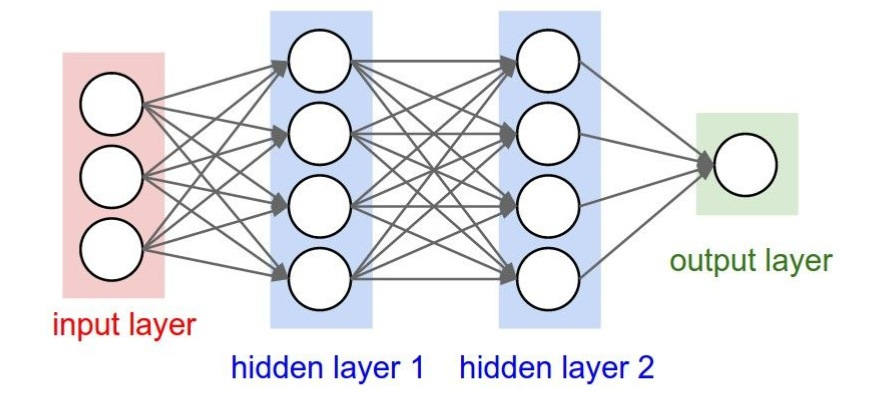
\includegraphics[width=0.45\textwidth]{Figures/2020-07-28-20-42-04.png}
        \caption{A Three-Layer Perceptron}
    \end{figure}
    \newpage
    \begin{itemize}
        \item \emph{Optimal Control.} \textit{Optimal control theory} is a branch of mathematical optimization that deals with finding a control for a dynamical system over a period of time such that an objective function is optimized. It has numerous applications in both science and engineering. For example, the dynamical system might be a spacecraft with controls corresponding to rocket thrusters, and the objective might be to reach the moon with minimum fuel expenditure. Or the dynamical system could be a nation's economy, with the objective to minimize unemployment; the controls in this case could be fiscal and monetary policy.
        \item \emph{Nonlinear Programming}
        \item \emph{Power System}
        \item \emph{Lagrangian Mechanics}
        \item \dots
    \end{itemize}
    In summary, as an engineer, we will face really complicated problems. It is a common situation where you need to deal with thousands of variables under hundreds of constraints. (Not a joke. Think about GPT-2, a language model with 1,500,000,000 parameters!) That's why a systematic method is in need.
\end{frame}

\section{Second Derivative and Extrema}
\begin{frame}
    \frametitle{Outline}
    \begin{spacing}{2.5}
        \tableofcontents[currentsubsection,hideothersubsections,sectionstyle=hide]
    \end{spacing}
\end{frame}

\subsection{Second Derivative}
\begin{frame}
    \frametitle{General Second Derivative}
    Let $X,V$ be finite-dimensional normed vector spaces and $\Omega\subset V$ an open set. A function $f:\Omega\to V$ is said to be \emph{twice dif{}ferentiable at $x\in\Omega$} if
    \begin{itemize}
        \item $f$ is dif{}ferentiable in an open ball $B_{\varepsilon}(x)$ around $x$ and
        \item the function $Df:B_\varepsilon(x)\to\mathcal{L}(X,V)$ is dif{}ferentiable at $x$.
    \end{itemize}
    We say that $f$ is twice dif{}ferentiable on $\Omega$ if $f$ is twice dif{}ferentiable at every $x\in\Omega$.\\[5pt]
    The derivative of $Df$ (if it exists) is a map
    \setcounter{equation}{0}
    \begin{equation}\label{2.5.1}
        D(Df)=:D^2f:\Omega\to\mathcal{L}(X,\mathcal{L}
        (X,V)).
    \end{equation}
    We call \eqref{2.5.1} the \emph{second derivative of $f$}. If the map $x\mapsto D^2f|_x$ is continuous on $\Omega$ we say that $f\in C^2(\Omega,V)$.
    \nullspace
    \textbf{Question}: What is essentially a second derivative? In other words, it is a function that maps what to what?
\end{frame}

\begin{frame}
    \frametitle{Exercise}
    Find the first and second derivative of
    \begin{itemize}
        \item $f(A)=A^3$,
        \item $g(A)=\operatorname{tr}(A^3)$.
    \end{itemize}
    \nullspace
    \textbf{Remark:} Although you can use chain rule to simplify the calculation, it is always a good choice to trust the definition.
\end{frame}

\begin{frame}[allowframebreaks]
    \frametitle{Second Derivative of Potential Function}
    We can write
    \[Df:x\mapsto(\nabla f(x))^T=Df|_x.\]
    Hence, $Df=(\,\cdot\,)^T\circ\nabla f$ and we can dif{}ferentiate $Df$ by the chain rule. The derivative of the map
    \[\nabla f:\R^n\to\R^n,\qquad\qquad\quad
        \nabla f(x)=\begin{pmatrix}
            \frac{\partial f}{\partial x_1}\big|_x \\
            \vdots                                 \\
            \frac{\partial f}{\partial x_n}\big|_x
        \end{pmatrix}\]
    \vspace*{-1pt}
    can be easily calculated: assuming suf{}ficient smoothness of $f$, it is just the Jacobian of $\nabla f$.
    \nullspace
    \textbf{Remark:} We represent $Df|_x$ using $\nabla f(x)$ because we are familiar with how to differentiate a column vector.
    \newpage
    We hence have
    \begin{equation}\label{2.5.2}
        D(\nabla f)|_x=\begin{pmatrix}
            \frac{\partial^2 f}{\partial x_1\partial x_1}\Big|_x & \frac{\partial^2 f}{\partial x_2\partial x_1}\Big|_x & \cdots & \frac{\partial^2 f}{\partial x_n\partial x_1}\Big|_x \\
            \vdots                                               & \vdots                                               & \ddots & \vdots                                               \\
            \frac{\partial^2 f}{\partial x_1\partial x_n}\Big|_x & \frac{\partial^2 f}{\partial x_2\partial x_n}\Big|_x & \cdots & \frac{\partial^2 f}{\partial x_n\partial x_n}\Big|_x
        \end{pmatrix}\in\text{Mat}(n\times n;\R).
    \end{equation}
    where
    \[\frac{\partial^2f}{\partial x_i\partial x_j}:=\frac{\partial}{\partial x_i}
        \frac{\partial f}{\partial x_j}\]
    is the second partial derivative of $f$ with respect to $x_j$ (first) and $x_i$ (second). The matrix in \eqref{2.5.2} is important enough to warrant a special name: It is called the \emph{Hessian} of $f$ and denoted by
    \[\text{Hess}\,f(x).\]
    \textbf{Remark:} Notice that Hessian is not the second derivative of $f$ at $x$. Instead, it is merely the first derivative of $\nabla f$ at $x$. We therefore need further calculation to figure out the second derivative of $f$ at $x$, and furthermore, how it operates.
    \newpage
    Recall that the transposition is a linear map, so its derivative is again the
    transposition. Hence,
    \begin{equation}\label{2.5.3}
        \begin{aligned}
            D^2f|_xh & =D((\,\cdot\,)^T\circ\nabla f(x))=D(\,\cdot\,)^T|_{\nabla f(x)}\circ D(\nabla f)|_xh \\
                     & =(\,\cdot\,)^T\circ D(\nabla f)|_xh=(\text{Hess}\,f(x)h)^T.
        \end{aligned}
    \end{equation}
    As required, $D^2f|_xh$ is a "row vector", i.e., an element of $\mathcal{L}(\R^n,\R)$. We see that if $\tilde{h}\in\R^n$ is some other vector, $D^2f|_xh$ acts on $\tilde{h}$ via
    \[(D^2f|_xh)\tilde{h}=(\text{Hess}\,f(x)h)^T\tilde{h}
        =\scp{\text{Hess}\,f(x)h}{\tilde{h}}\in\R.\]
    Note that the expression $\scp{\text{Hess}\,f(x)h}{\tilde{h}}$ is linear in both $h$ and $\tilde{h}$; hence we can also regard the second derivative as a \emph{bilinear map}
    \[D^2f|_x:\R^n\times\R^n\to\R,\qquad\qquad
        (h,\tilde{h})\mapsto\scp{\text{Hess}\,f(x)h}{\tilde{h}}.\]
    \textbf{Remark:} What is $D^2f|_x, D^2f|_xh,(D^2f|_xh)\tilde{h}$ respectively?
\end{frame}

\begin{frame}
    \frametitle{Bilinear Map}
    The second derivative is a bilinear map. We have learned general multi-linear map in the lecture, but now let's focus on the form of linear and bilinear map.
    \begin{itemize}
        \item
              All linear maps in the form $\R^n\to\R$ can be represent using a $1\times n$ matrix $L$ (i.e. a row vector, or an element in dual space of $\R^n$). Moreover, it operates via $Lx$, or $\langle L^T,x \rangle$.
        \item
              \[\mathcal{L}(X,\mathcal{L}(X,V))\cong
                  \mathcal{L}^{(2)}(X,V).\]All bilinear maps in the form $\R^n\times\R^n\to \R$ can be represent using a $n\times n$ matrix $A$. Moreover, it operates via $\langle Ay,x \rangle$, or equivalently, $(Ay)^Tx$.
    \end{itemize}
\end{frame}

\begin{frame}
    \frametitle{Schwarz's Theorem}

    If $f:\R^n\to\R$ is twice dif{}ferentiable, we can represent $D^2f$ in the form of a square $n\times n$ matrix; this is just the Hessian we have introduced in \eqref{2.5.2}.
    However, in general we can not represent the second derivative of a
    function $\R^n\to\R^m$ as a matrix; furthermore, even in the case of potential functions $(m=1)$ higher order derivatives can not be expressed as matrices.\\[6pt]
    \emph{Schwarz's Theorem.} Let $X,V$ be normed vector spaces and $\Omega\subset X$ an open set. Let $f\in C^2(\Omega,V)$. Then $D^2f|_x\in\mathcal{L}^{(2)}(X\times X,V)$ is symmetric for all $x\in\Omega$, i.e.,
    \[D^2f(u,v)=D^2f(v,u),\qquad\qquad\quad
        \text{for all}~u,v\in X.\]

    \textbf{Remark:} In the case of potential functions $(X=\R^n,V=\R)$, it implies that
    \[\scp{\text{Hess}\,f(x)y}{z}=\scp{\text{Hess}\,f(x)z}{y},
        \qquad\qquad x,y,z\in\R^n.\]
    which means $\text{Hess}\,f(x)=(\text{Hess}\,f(x))^T$, i.e., the Hessian of $f$ at $x$ is a symmetric matrix. Writing out the components of $\text{Hess}\,f(x)$, this means that
    \[\frac{\partial^2f}{\partial x_i\partial x_j}=\frac{\partial^2f}{\partial x_j\partial x_i}.\]
    In other words, if $f$ is twice continuously dif{}ferentiable, the order of
    dif{}ferentiation in the second-order partial derivatives does not matter.
\end{frame}

\subsection{Free Extrema}
\begin{frame}
    \frametitle{Free Extrema}
    We now discuss the extrema of a potential function without any constraints. To do so, we need turn to quadratic approximation just like what we have done to find an extrema of functions in VV186. (Recall Taylor's Theorem.)
    \nullspace
    \emph{Quadratic Approximation.} Let $\Omega\subset\R^n$ be an open set and $f\in C^2(\Omega,\R)$. Then for any $h\in\R^n$ small enough that $x+h\in\Omega$,
    \begin{equation}\label{2.6.2}
        f(x+h)=f(x)+\scp{\nabla f(x)}{h}+\int_{0}^{1}(1-t)\scp{\text{Hess}\,f(x+th)h}{h}dt.
    \end{equation}
    \emph{Corollary.} Let $\Omega\subset\R^n$ be an open set and $f\in C^2(\Omega,\R)$. Then, as $h\to0$,
    \begin{equation}\label{2.6.3}
        f(x+h)=f(x)+\scp{\nabla f(x)}{h}+\frac{1}{2}\scp{\text{Hess}\,f(x)h}{h}+o(h^2).
    \end{equation}
    \textbf{Remark:} At the extrema point, the second item of Eq.\ref{2.6.3} vanishes for all directions. Then the variation trend of the function is dominated by the third item. You can make a comparison of it with what we have learned in VV186.
\end{frame}

\begin{frame}[allowframebreaks]
    \frametitle{Quadratic Forms}
    To better deal with the third item $\scp{\text{Hess}\,f(x)h}{h}$, we introduce \emph{quadratic form}.\nullspace
    Let $A\in\text{Mat}(n\times n,\R)$. Then the \emph{quadratic form induced by $A$} is defined as the map
    \[Q_A:=\scp{\cdot}{A(\,\cdot\,)},\qquad
        x\mapsto\scp{x}{Ax}=\sum_{j,k=1}^{n}a_{jk}x_jx_k,
        \qquad x\in\R^n.\]
    Clearly, $Q_A(\lambda x)=\lambda^2Q_A(x)$ for any $\lambda\in\R$. Note also that $Q_A$ is continuous, because it is a polynomial in \myseries{x}{n}.\\[8pt]
    \emph{Definition.} A quadratic form $Q_A$ induced by a matrix $A\in\text{Mat}(n\times n,\R)$ is called
    \begin{itemize}
        \item \emph{positive definite} if $Q_A(x)>0$ for all $x\neq0$,
        \item \emph{negative definite} if $Q_A(x)<0$ for all $x\neq0$,
        \item \emph{indefinite} if $Q_A(x_0)>0$ for some $x_0\in\R^n$ and $Q_A(y_0)<0$ for some $y_0\in\R^n$.
    \end{itemize}
    A matrix $A$ is said to be negative definite / positive definite / indefinite if the induced quadratic form $Q_A$ has the corresponding property.
    \newpage
    \textbf{Remark:}
    \begin{itemize}
        \item It is easy to see that not all quadratic forms fall into one of the above
              three categories.
        \item If $A$ is positive definite, then $-A$ is negative definite.
    \end{itemize}
    \nullspace
    A particular case in $\R^2$:\\[8pt]
    Let $A\in\text{Mat}(2\times 2,\R)$ be symmetric, i.e.,
    \[A=\begin{pmatrix}
            a & b \\
            b & c
        \end{pmatrix}.\]
    Let $\Delta=\det A$. Then
    \begin{itemize}
        \item[(i)] $A$ positive definite $\Rightarrow$ $a>0$ and $\Delta>0$
        \item[(ii)] $A$ negative definite $\Rightarrow$ $a<0$ and $\Delta>0$
        \item[(iii)] $A$ indefinite $\Rightarrow$ $\Delta<0$
    \end{itemize}
\end{frame}

\begin{frame}
    \frametitle{Local \& Global, Maximum \& Minimum}
    Let $\Omega\subset\R^n$ and $f:\Omega\to\R$.

    \begin{enumerate}[(i)]
        \item $f$ is said to have a \emph{(global) maximum} at $\xi\in\Omega$ if
              \[x\in\Omega\qquad\Rightarrow\qquad
                  f(x)\leq f(\xi).\]
        \item $f$ is said to have a \emph{strict (global) maximum} at $\xi\in\Omega$ if
              \[x\in\Omega\setminus\{\xi\}\qquad\quad
                  \Rightarrow\qquad\quad f(x)<f(\xi).\]
        \item $f$ is said to have a \emph{local maximum} at $\xi\in\Omega$ if there exists a $\delta>0$ such that
              \[x\in\Omega\cap B_\delta(\xi)\qquad\Rightarrow\qquad
                  f(x)\leq f(\xi).\]
        \item $f$ is said to have a \emph{strict local maximum} at $\xi\in\Omega$ if there exists a $\delta>0$ such that
              \[x\in\Omega\cap B_\delta(\xi)\setminus\{\xi\}\qquad
                  \Rightarrow\qquad f(x)<f(\xi).\]
    \end{enumerate}
    The function $f$ is said to have a (strict) global/local minimum at $\xi$ if $-f$ has a (strict) global/local maximum at $\xi$.
\end{frame}

\begin{frame}
    \frametitle{Finding Extrema}
    \emph{Essential Condition.} Let $\Omega\subset\R^n,f:\Omega\to\R$ and $\xi\in\text{int}\,\Omega$. Assume that all partial derivatives of $f$ exist at $\xi$ and that $f$ has a local extremum (maximum or minimum) in $\xi$. Then
    \[\nabla f(\xi)=0.\]
    If $f$ is dif{}ferentiable in $\xi$, this implies $Df|_\xi=0$.
    \nullspace
    \emph{Hessian \& Extrema} Let $\Omega\subset\R^n$ be open, $f\in C^2(\Omega)$ and $\xi\in\Omega$. Let $\nabla f(\xi)=0$ (i.e., $Df|_\xi=0$).
    \begin{enumerate}[(i)]
        \item If Hess $f|_\xi$ is positive definite, $f$ has a strict local minimum at $\xi$.
        \item If Hess $f|_\xi$ is negative definite, $f$ has a strict local maximum at $\xi$.
        \item If Hess $f|_\xi$ is indefinite, $f$ has no extremum at $\xi$.
    \end{enumerate}
    \vspace{8pt}
    \textbf{Remark:} We often call $\xi\in\operatorname{int}\,\Omega$ the critical points. Notice that a local extremum can exist at the boundary of $\Omega$ without being a critical point. Additionally, The second theorem gives us a practical way to tell whether a critical point is an extremum.
\end{frame}

\begin{frame}
    \frametitle{Critical Point}
    A critical point is not necessarily an extrema. $(0,0)$ is critical point for both of the functions below. However, it is merely a \emph{saddle point}.
    \begin{columns}
        \begin{column}{0.5\textwidth}
            \begin{figure}[H]
                \centering
                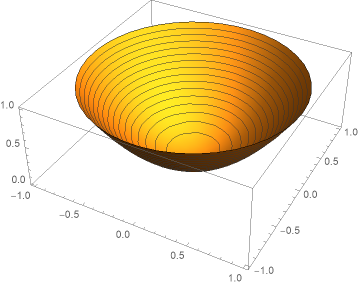
\includegraphics[width=\textwidth]{Figures/2020-07-29-15-39-20.png}
                \caption{$z=x^2+y^2$}
            \end{figure}
        \end{column}
        \begin{column}{0.5\textwidth}
            \begin{figure}[H]
                \centering
                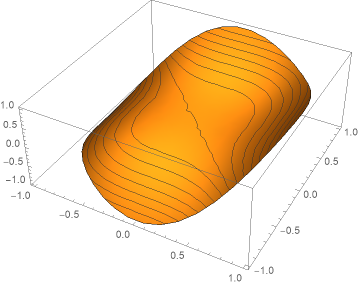
\includegraphics[width=\textwidth]{Figures/2020-07-29-15-40-05.png}
                \caption{$z=x^3+y^3$}
                \label{fig:}
            \end{figure}

        \end{column}
    \end{columns}
\end{frame}

\begin{frame}
    \frametitle{General Procedure}
    We follow a four-step process to find the extrema of a potential function $f\in\C^2(\Omega,\R)$.
    \begin{itemize}
        \item[1.] Check for critical points $\xi\in\text{int}\,\Omega$, i.e., those were $Df|_\xi=0$.
        \item[2.] Use Theorem 2.6.12 or Corollary 2.6.13 to check which of the critical points is an extremum.
        \item[3.] Check the boundary $\partial\Omega$ separately for local extrema.
        \item[4.] Identify the global extrema. Any finite global extremum must also be
              a local extremum, so it will be included among those found above.
    \end{itemize}

    \textbf{Remark:} For Step 3, we are not really going to find the local extrema. Instead, we are just looking for candidates for global extrema. An example is shown later to illustrate it.
\end{frame}

\begin{frame}
    \frametitle{Exercise}
    Consider the following function:
    \[
        \begin{array}{c}
            g: \mathbb{R}^{2} \rightarrow \mathbb{R} \\
            g(x, y):=x^{3}- y^{2}-xy+1
        \end{array}
    \]
    Find its  extrema.
    \pause

    \begin{figure}[H]
        \centering
        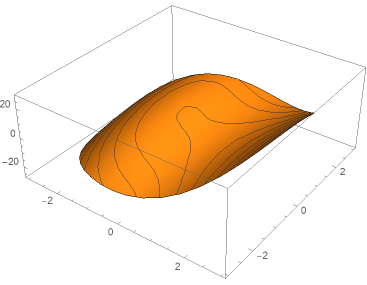
\includegraphics[width=0.5\textwidth]{Figures/2020-07-29-15-59-00.png}
    \end{figure}

\end{frame}

\begin{frame}
    \frametitle{Exercise}
    Consider the following function:
    Find its global extrema.
    \[
        \begin{array}{c}
            f: \Omega \subset \mathbb{R}^{2} \rightarrow \mathbb{R} \\
            f(x, y):=x^{3}+2 y^{2}+1
        \end{array}
    \]
    where $\Omega=B[0,3]=\left\{(x, y) \in \mathbb{R}^{2}: x^{2}+y^{2} \leq 9\right\}$

    \pause

    \begin{figure}[H]
        \centering
        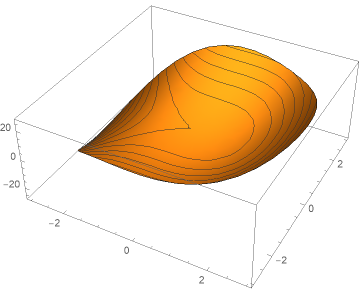
\includegraphics[width=0.5\textwidth]{Figures/2020-07-29-15-52-27.png}
    \end{figure}
\end{frame}

\begin{frame}[allowframebreaks]
    \frametitle{Local Extremum at Boundary}
    When we want to find the global extrema of a function on some region $\Omega$, we don't bother to judge whether a critical point at the boundary is a local extrema or not. What we do is just find its value, and make a comparison with other candidates. However, things become more tricky if we want to find all the local extrema including points at the boundary.
    \begin{figure}[H]
        \centering
        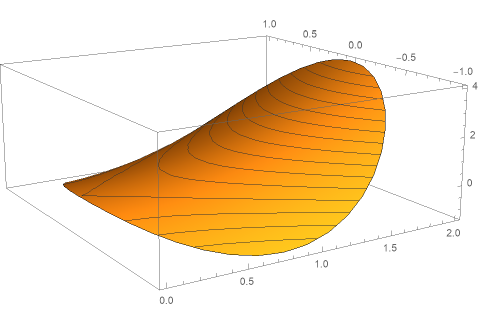
\includegraphics[width=0.5\textwidth]{Figures/2020-07-29-15-28-47.png}
        \caption{Potato Chip}
    \end{figure}

    \newpage
    At this moment, we can either use the definition of local extrema, or use this theorem to deduce a point on the boundary is a extrema:
    $$
        f(x+h)=f(x)+\scp{\nabla f(x)}{h}+\frac{1}{2}\scp{\text{Hess}\,f(x)h}{h}+o(h^2).
    $$

\end{frame}

\subsection{Constrained Extrema}
\begin{frame}
    \frametitle{Constrained Extrema}
    Constrained extrema is a very important topic in this part. While implicit function theorem is very interesting, we will focus on the lagrange multiplier rule, which is a more practical method to solve constrained extrema problems.
    \nullspace
    Let $\Omega \subset R^{n}$ be open and $F \in C^{p}\left(\Omega, \mathbb{R}^{m}\right), p \geq 1,$ such that $F(\xi)=0$ for some $\xi=\left(\xi^{\prime}, \xi^{\prime \prime}\right) \in \Omega, \xi^{\prime}=\left(\xi_{1}, \cdots, \xi_{m}\right) .$ Assume further that
    \[
        \left.\operatorname{det} D F\left(\cdot, \xi^{\prime \prime}\right)\right|_{\xi^{\prime}} \neq 0
    \]
    Then there exists an open ball $B_{\varepsilon}\left(\xi^{\prime \prime}\right)$ and a $C^{p}$ -map $g: B_{\varepsilon}\left(\xi^{\prime \prime}\right) \rightarrow \mathbb{R}^{m}$
    such that
    \[
        F\left(x^{\prime \prime}, g\left(x^{\prime \prime}\right)\right)=0 \quad \text { for all } x^{\prime \prime} \in B_{\varepsilon}\left(\xi^{\prime \prime}\right)
    \]
    The derivative of $g$ is given by
    \[
        \left.D g\right|_{x^{\prime \prime}}=-\left.\left(\left.D F\left(\cdot, x^{\prime \prime}\right)\right|_{g\left(x^{\prime \prime}\right)}\right)^{-1} D F\left(g\left(x^{\prime \prime}\right), \cdot\right)\right|_{x^{\prime \prime}}
    \]
\end{frame}

\begin{frame}
    \frametitle{Exercise}

    For implicit function $x^2+y^2+z^2=4z$, find $\dfrac{\partial z}{\partial x}$, $\dfrac{\partial z}{\partial y}$. (What is the tangent vectors of the tangent surface at some point $(x,y,z)$?)

\end{frame}

\begin{frame}[allowframebreaks]
    \frametitle{Lagrange Multiplier Rule}

    Let $\Omega\subset\R^n$ be open and $f\in C^1(\Omega,\R),g\in C^1(\Omega,\R^m),m<n$. Assume that $f$ has a local extremum on the set $E=\{x\in\R^n:g(x)=0\}$ at $\xi\in E$. Assume further that in
    \[Dg|_\xi=\begin{pmatrix}
            \frac{\partial g_1}{\partial x_1} & \cdots & \frac{\partial g_1}{\partial x_n} \\
            \vdots                            & \ddots & \vdots                            \\
            \frac{\partial g_m}{\partial x_1} & \cdots & \frac{\partial g_m}{\partial x_n}
        \end{pmatrix}\]
    \textbf{there exists a submatrix consisting of $m$ columns whose determinant does
        not vanish}. Then there exist $m$ numbers (called Lagrange multipliers) \myseries{\lambda}{m}$\in\R$ such that
    \begin{equation}\label{2.7.4}
        Df|_\xi+\sum_{i=1}^{m}\lambda_i Dg_i|_\xi=0.
    \end{equation}

    In order to find the constrained extrema, we need to solve the $m + n$ equations
    \begin{align*}
        \frac{\partial f}{\partial x_i}+\lambda_1\frac{\partial g_1}{\partial x_1}+\cdots+\lambda_m\frac{\partial g_m}{\partial x_i} & =0,\qquad\qquad i=1,\ldots,n, \\
        g_j(x)                                                                                                                       & =0,\qquad\qquad j=1,\ldots,m.
    \end{align*}
    These equations are equivalent to the following: define
    \[F(x_1,\ldots,x_n,\lambda_1,\ldots,\lambda_m)
        :=f(x)+\lambda_1g_1(x)+\cdots+\lambda_mg_m(x).\]
    Then at an extremal point all partial derivatives of $F$ will vanish.
\end{frame}

\begin{frame}
    \frametitle{Exercise}
    Example Suppose the unit sphere centered at the origin in $\mathbb{R}^{3}$ is heated so that its temperature at a point is given by
    \[
        T(x, y, z)=80+50(x+z)
    \]
    Suppose we wish to find the extreme values of $T$ along the intersection $D$ of the sphere with the plane $x+y+z=1$ (see the picture below). That is, we wish to find the extrema of $T$ subject to the constraints
    \[
        x^{2}+y^{2}+z^{2}=1
    \]
    and
    \[
        x+y+z=1
    \]

\end{frame}

\begin{frame}
    \frametitle{Application: Optics}
    Let's use \textit{Lagrange multiplier rule} and \textit{Fermat's principle} to deduce the \textit{law of refraction}.
    $$n_1\sin\theta_1=n_2\sin\theta_2.$$
    \href{https://en.wikipedia.org/wiki/Fermat\%27s_principle}{Fermat's principle.} The light travels the path which takes the least time. \footnote[frame]{This statement is simplified. In order to be true in all cases, it must be weakened by replacing the "least" time with a time that is "stationary" with respect to variations of the path — so that a deviation in the path causes, at most, a second-order change in the traversal time.}
    \begin{figure}[H]
        \centering
        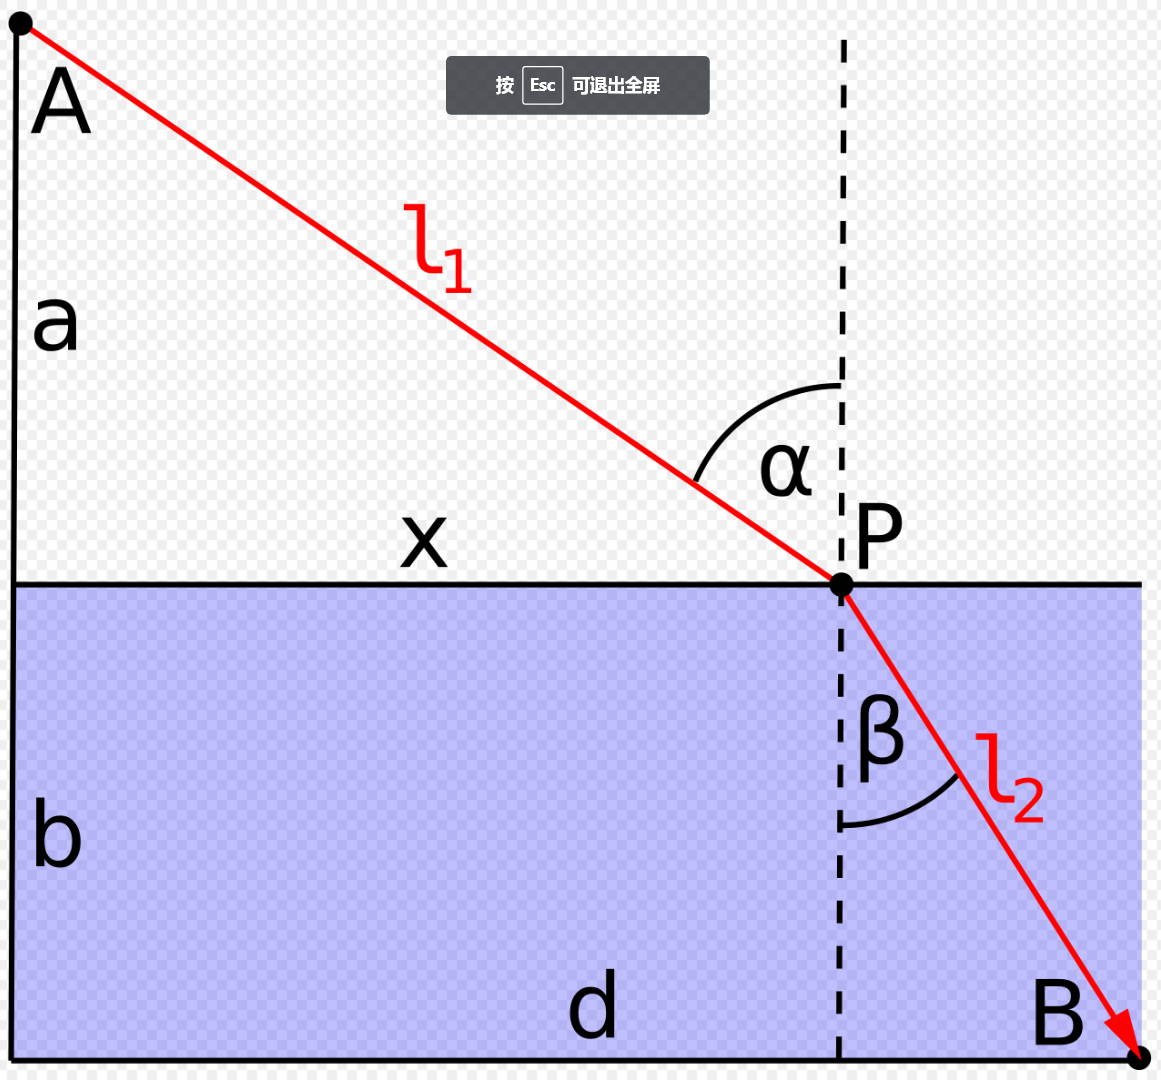
\includegraphics[width=0.3\textwidth]{Figures/2020-07-29-16-52-32.png}
        \caption{Refraction}
    \end{figure}
\end{frame}

\begin{frame}
    \frametitle{Summary}

    I would like to express my gratitude to all of you. Thank you for coming to my last regular RC and make this experience a meaningful journey for me, and hopefully, for you too.\\[8pt]
    Mathematics is so beautiful and mysterious. I am marvelled by her again and again in my own study. And that's why I planned to be a TA of VV285. Trust me, it's very tough. I need to spend two days a week grading assignments, preparing RC and answering questions on piazza. But it is worthwhile -- I cannot feel more meaningful to share my own understanding and happiness to you, and help some of you recognize the wonderfulness of mathematics rather than a fear of it. I hope this journey really make some difference.
    \\[8pt]
    However, as future engineers, I hope you understand math is not an isolated discipline. It has innumerable links with other subjects. That's why I put much effort on finding relevant examples regarding electromagnetics, fluid dynamics, optics, computer science, and etc. I hope you can continue building an interdisciplinary spirit afterwards.
    \\[8pt]
    Time to end. Thank you again!
\end{frame}

\begin{frame}
    \frametitle{Discussion}
    \vspace{1cm}
    \begin{center}
        \LARGE
        Forever\\
        Have Fun\\
        And\\
        Learn Well!
    \end{center}
\end{frame}

\end{document}